\documentclass[12pt,letterpaper,twocolumn]{article}
\usepackage[utf8]{inputenc}
\usepackage[spanish,es-tabla]{babel}
\decimalpoint
\let\cleardoublepage\clearpage
% \usepackage[bitstream-charter]{mathdesign}
% \usepackage[T1]{fontenc}
% \newcommand{\selectSans}{\usefont{T1}{qhv}{m}{n}\selectfont} % sans-serif TeX Gyre Heros font
\usepackage{amsmath}
\usepackage{amsfonts}
\usepackage{amssymb}
\usepackage{blindtext}
\setlength{\columnseprule}{0.2pt}
% \usepackage[T1]{fontspec}
\usepackage{color}
\usepackage{makeidx}
\usepackage{enumitem}
\usepackage{float}
\usepackage{graphicx}
\usepackage{subcaption}
\makeindex
\usepackage{anysize}
\usepackage{anyfontsize}
\usepackage{pdfpages}
\usepackage[x11names,table]{xcolor}
\usepackage{tikz}
\usepackage{tcolorbox}
\tcbuselibrary{skins,breakable,listings,theorems}
\usepackage[hidelinks]{hyperref}
\usepackage[labelfont=bf]{caption}
\captionsetup[table]{labelsep=space}
\captionsetup[figure]{labelsep=space}
\usepackage{listings}
\usepackage{array,ragged2e}
\usepackage{multirow}
\usepackage[left=2cm,top=2cm,right=2cm,bottom=2cm]{geometry}
\setlength{\parindent}{0cm}
% \usepackage[printwatermark]{xwatermark}
% \newwatermark[allpages,color=gray!10,angle=45,scale=3,xpos=0,ypos=0]{Borrador}
\tcbset{colback=green!5!white, colframe=gray!10!black, coltitle=green!20!black, 
fonttitle=\bfseries, colbacktitle=white, coltext=gray!30!black}
\addto\captionsspanish{
  \renewcommand{\figurename}{{\bf Figura}}% 
}
\addto\captionsspanish{
  \renewcommand{\chaptername}{{\bf}}% 
}

\usepackage{epigraph}
\usepackage{fontawesome}
% \usepackage[Bjornstrup]{fncychap}

% \renewcommand{\familydefault}{\sfdefault}

% Colores
\definecolor{verdep}{RGB}{166,206,58}
\definecolor{ccap}{RGB}{10,10,50}
\definecolor{csec}{RGB}{50,50,100}
\definecolor{csubsec}{RGB}{80,80,120}
\definecolor{header_table_color}{RGB}{200,255,180}
\definecolor{info_color}{RGB}{100,100,200}
\definecolor{csol}{rgb}{0.2,0.8,0.1}
\definecolor{backcode}{rgb}{0.98,0.98,0.99}
\definecolor{crule}{rgb}{0.9,0.9,0.9}
\definecolor{dkgreen}{rgb}{0,0.6,0}
\definecolor{gray}{rgb}{0.5,0.5,0.5}
\definecolor{mauve}{rgb}{0.58,0,0.82}

\newtcolorbox{informacion}[2][]
{
  breakable,
  colframe = blue!5!white,
  colback  = blue!5!white,
  coltitle = blue!80!black,
  title    = \faInfo \hspace{5 mm} #2,
}

\newcommand{\puntos}[1]{ {\small\sffamily [#1 \%]} }

\newcommand{\ccol}{>{\centering\tt\arraybackslash}}

% Code
\lstnewenvironment{matlab}{\lstset{frame=single,
  frameround=tttt,
  backgroundcolor=\color{backcode},
  rulecolor=\color{crule},
  language=matlab,
  aboveskip=5mm,
  belowskip=5mm,
  showstringspaces=false,
  columns=flexible,
  basicstyle={\small\ttfamily},
  numbers=none,
  numberstyle=\tiny\color{gray},
  keywordstyle=\color{blue},
  commentstyle=\color{dkgreen},
  stringstyle=\color{mauve},
  breaklines=true,
  breakatwhitespace=true,
  tabsize=4,
  extendedchars=true,
  inputencoding=utf8,
  literate=%
  {°}{{\,\,$^\circ$\,\,}}1
  {á}{{\'a}}1
  {é}{{\'e}}1
  {í}{{\'i}}1
  {ó}{{\'o}}1
  {ú}{{\'u}}1
  {Á}{{\'A}}1
  {É}{{\'E}}1
  {Í}{{\'I}}1
  {Ó}{{\'O}}1
  {Ú}{{\'U}}1
}}{}


\author{}
\date{}
\title{
\vspace{-20mm}
{\normalsize Instituto Tecnológico de Celaya} \\ [-3.5mm]
{\normalsize Ingeniería Mecatrónica} \\ [-3.5mm]
{\normalsize Mecánica de Materiales} \\ [-3.5mm]
{\bf\normalsize Examen Unidad I. Esfuerzo y deformación} \\ [2mm]
{\normalsize Nombre: \rule{8cm}{0.4pt} \hfill Fecha: \rule{3cm}{0.4pt} }
}


\begin{document}
\maketitle
\vspace{-20mm}

\textbf{1.}  Sabiendo que el eslabón DE tiene 1/8 in de espesor y 1 in de ancho, calcule el esfuerzo normal 
en la porción central del eslabón cuando a) $\theta=0$° b) $\theta=90$°.  \puntos{30} \\[-2mm]

\begin{center}
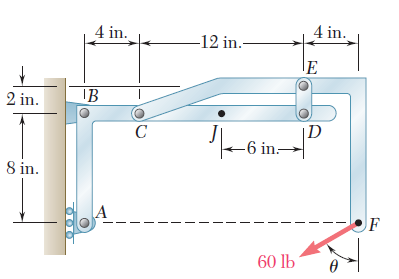
\includegraphics[width=0.45\textwidth]{img/p01.PNG}
\end{center}


\textbf{2.} El eslabón AB, de ancho $b=50\text{ mm}$  y espesor $t=6\text{ mm}$, es utilizado para 
cargar el extremo de una viga horizontal. Sabiendo que el esfuerzo normal promedio en el eslabón es 
de -140 MPa, y que el esfuerzo cortante promedio en cada uno de los dos pernos es de 80 MPa, calcule 
a) el diámetro $d$ de los pernos b) el esfuerzo de apoyo en el elemento. \puntos{30}

\begin{center}
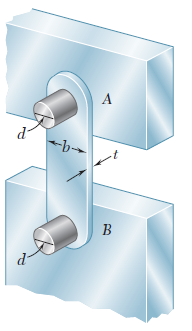
\includegraphics[width=0.20\textwidth]{img/p02.PNG}
\end{center}

\textbf{3. } El segmento AB de la barra es un tubo con un diámetro exterior de 1.5 in y un espesor 
de pared de 0.125 in. El segmento BC es una barra solida de diámetro 0.75 in. Calcule el esfuerzo normal 
en cada segmento y su deformación unitaria, considerando que el material para ambos segmentos es un 
acero. \puntos{30}

\begin{center}
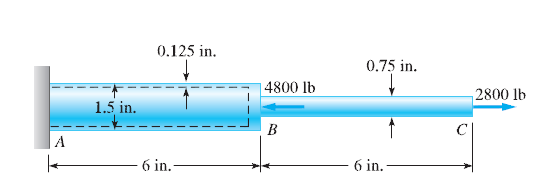
\includegraphics[width=0.55\textwidth]{img/p03.PNG}
\end{center}

\textbf{4. } Describa, de manera breve pero concisa, el concepto de factor de seguridad. \puntos{10}


\end{document}